\documentclass[notitlepage]{report}
\usepackage{graphicx}
\usepackage[left=1in, right=1in, top=1in, bottom=1in]{geometry}
\usepackage[spanish]{babel}
\selectlanguage{spanish}
\spanishdecimal{.}
\usepackage[utf8]{inputenc}
    
\usepackage{titling}
\usepackage{lipsum}

\pretitle{\begin{center}\Huge\bfseries}
\posttitle{\par\end{center}\vskip 0.5em}
\preauthor{\begin{center}\Large\ttfamily}
\postauthor{\end{center}}


\title{Python y Jupyter Notebooks}
\author{Borbón Fragoso Julio César\\ \\
\small{Grupo 1 Física computacional}\\
\small{}\\
\small}


\begin{document}

\maketitle

\section*{1.-Introducción}
Python es un lenguaje de programación intrepetado, esto quiere decir que ejecuta lineas de codigo a medida que sea necesario, es de uso libres y es uno de los más usados a nivel mundial. 
Existen varios tipos de entornos para poder usar Python, uno de ellos es Jupyter Notebooks también de uso libre y un lugar viable para programar en Python. \\ 
Para hacer las cosas más sencillas y útiles a la hora de trabajar en Python tenemos librerias que amplian las funciones que tiene el lenguaje de programación, por ejemplo existe una llamada Panda, que nos da la facilidad de manejar datos de forma muy parecida a un lenguaje enfocado en el manejo de datos como R, también existe Numerycal Python que a mi parecer tiene un potencial de uso en el área de física ya que añade funciones que nos permiten manejar de mejor manera vectores y matrices.  Por último tenemos a Matplotlib que tiene como propósito ampliar la útilidad gráfica del lenguaje.


\section*{2.- Usando Python}
Para útilizar por primera vez Python se pidío emular un codigo ya hecho con nuestros propios datos, estos datos tenían que venir del servicio metereológico  nacional con una función llamada "Estaciones Metereológicas Automáticas" mi elección fue la ciudad de la piedad en el estado de Michoacan  \\
A continuación se presenta cierta información obtenida durante la actividad realizada: \\ 

   
     \includegraphics[scale=.85]{imagen1.png}\\
  \includegraphics[scale=.85]{Imagen3.png}\\
  \includegraphics[scale=.85]{Imagen2.png}\\
  \includegraphics[scale=.85]{Imagen4.png}}\\
    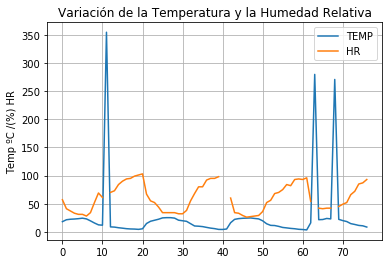
\includegraphics[scale=.85]{index.png}\\
      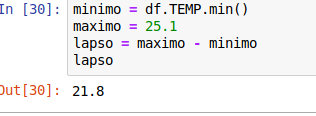
\includegraphics[scale=.85]{tempmrdia.png}\\
      
      Se pueden observar en los gráficos que las rafagas predominan sobre el viento y que cuando la temperatura incrementa la humedad relativa disminuye. Además el lapso de temperatura es de 21.8, se solicito una gráfica de la radiación solar sin embargo la tabla descargada no tenía datos sobre esto.  \\
      
      \section*{3.- Anexo}
      
      Se anexan las siguientes preguntas: \\
      ¿Cuál es tu primera impresión de Jupyter Notebook? \\
      {\bfseries Me fue agradable de usar, sencillo con los atajos que necesite y no tuve complicaciones} \\
      
     ¿Se te dificultó leer código en Python? \\ 
      {\bfseries La mayor parte me parecio intuitiva, sin embargo otra se me hizo muy extraña} \\
      
     ¿En base a tu experiencia de programación en Fortran, que te parece el entorno de trabajar en Python? \\ 
     {\bfseries Pude notar que con una cantidad menor de instrucciones podías hacer cosas que con Fortran originalmente hubiera tardado más, me parece que Python es diferente a Fortran y en la actualidad creo que me sería más útil Python que Fortran} \\
     
     A diferencia de Fortran, ahora se producen las gráficas utilizando la biblioteca Matplotlib. ¿Cómo fue tu experiencia?. \\
     {\bfseries Me gusto ver como se pueden generar gráficas de manera rapida con instrucciones sencillas } \\
     
     En general, ¿qué te pareció el entorno de trabajo en Python? \\
     {\bfseries Resumiendo: Bueno} \\
     
     ¿Qué opinas de la actividad? ¿Estuvo compleja? ¿Mucho material nuevo? ¿Que le faltó o que le sobró? ¿Qué modificarías para mejorar? \\
     {\bfseries Estuvo bastan bien, el único problema que se me presento fue la obtención de datos en la página del SMN, escogi varias localidades y carecian de datos suficientes para satisfacer la actividad, al final escogi un lugar con suficiente datos pero aun así no proporcionaba nada sobre la radiación solar}
     
     






      
      





\end{document}
